\documentclass[12pt]{article}
\usepackage[a4paper,left=1in,right=1in, top=1in, bottom=1in]{geometry}
% marginleri 1er inch yaptim
\renewcommand{\baselinestretch}{1.15} % satir araligi 1.15
% \usepackage{mathptmx}
\usepackage{subfig}
% \usepackage[utf8]{inputenc}
\usepackage[style=ieee]{biblatex}
%\usepackage[document]{ragged2e}
\usepackage{titlesec}
%\usepackage{hyperref}
%\usepackage{setspace}
% \usepackage{amsmath}
\usepackage{graphicx}
\graphicspath{{./images/}}
% \usepackage{makeidx}
% \usepackage{rotating}
% \usepackage{tikz}
\usepackage{array}
\usepackage{acronym}
\usepackage{draftwatermark}
% \usepackage[pages=some]{background}
\SetWatermarkText{
\includegraphics[angle=-45]{watermark.png}}
% BU watermark iyi duruyor mu?
% watermark icin
\usepackage{hyperref}
% \usepackage{float}
\usepackage{adjustbox}
% \usepackage{times}
\usepackage{fontspec}
\setromanfont{Times New Roman}
% \usepackage{ragged2e}
% \justifying
\usepackage{caption}
\usepackage{filecontents}
\captionsetup[table]{name=Tablo}
\renewcommand{\figurename}{Şekil}
\renewcommand{\contentsname}{İçindekiler}
\renewcommand{\listfigurename}{Şekiller Listesi}
\renewcommand{\listtablename}{Tablolar Listesi}

\addbibresource{references.bib}
%\renewcommand\refname{New Title}
% \selectlanguage{turkish}
\newcommand{\HRule}[1]{\rule{\linewidth}{#1}}
%\newcommand{\HRule}{\rule{\linewidth}{0.5mm}}

% \subsubsubsection ekleme kodu başlangıcı.
\titleclass{\subsubsubsection}{straight}[\subsection]

\newcounter{subsubsubsection}[subsubsection]
\renewcommand\thesubsubsubsection{\thesubsubsection.\arabic{subsubsubsection}}
\renewcommand\theparagraph{\thesubsubsubsection.\arabic{paragraph}} % optional; useful if paragraphs are to be numbered

\titleformat{\subsubsubsection}
  {\normalfont\small\bfseries}{\thesubsubsubsection}{1em}{}
\titlespacing*{\subsubsubsection}
{0pt}{3.25ex plus 1ex minus .2ex}{1.5ex plus .2ex}

\makeatletter
\renewcommand\paragraph{\@startsection{paragraph}{5}{\z@}%
  {3.25ex \@plus1ex \@minus.2ex}%
  {-1em}%
  {\normalfont\normalsize\bfseries}}
\renewcommand\subparagraph{\@startsection{subparagraph}{6}{\parindent}%
  {3.25ex \@plus1ex \@minus .2ex}%
  {-1em}%
  {\normalfont\normalsize\bfseries}}
\def\toclevel@subsubsubsection{4}
\def\toclevel@paragraph{5}
\def\toclevel@paragraph{6}
\def\l@subsubsubsection{\@dottedtocline{4}{7em}{4em}}
\def\l@paragraph{\@dottedtocline{5}{10em}{5em}}
\def\l@subparagraph{\@dottedtocline{6}{14em}{6em}}
\makeatother


\setcounter{secnumdepth}{4}
\setcounter{tocdepth}{4}
% \subsubsubsection ekleme kodu sonu.


\begin{document}

\title{\vspace{1cm}
% TARIH EKLENECEK MI
\textsc{\LARGE TEKNOFEST}\\[0.5cm]
\textsc{\large HAVACILIK, UZAY VE TEKNOLOJİ FESTİVALİ}\\[0.5cm]
\textsc{\large İnsansız Su Altı Sistemleri Yarışması}\\[0.5cm]

% i ler ı olmuş sorun olur mu?
% Ertuğrul: bence sorun yok göremedim bir şey.
\HRule{0.5pt} \\[0.4cm]
{\LARGE \bfseries ÖN TASARIM RAPORU}\\[0.3cm]
\HRule{0.5pt} \\[0.5cm]
{\large 25 Mart 2020}\\
% LOGO GELECEK
%\includegraphics{logo.png}\\[1cm]
\date{}
\author{

%Alt Alta:
%\textbf{Takım Adı}       &   Nucleo\\[10pt]
%\textbf{Takım ID}        &   T3-16167-166\\[10pt]
%\textbf{Takım Üyeleri}   &   Ege Saygılı, Enes Demirağ, Sencer Yazıcı, Sinan Ertuğrul Yıldırım\\[10pt]
%\textbf{Takım Danışmanı} &   Ar. Gör. Mehmet Ozan Şerifoğlu 

%Yan Yana:
\begin{tabular}{l|l}
\textbf{Takım Adı:}       &   Nucleo\\
\textbf{Takım ID:}        &   T3-16167-166\\
\textbf{Takım Üyeleri:}   &   Ege Saygılı\\
                          &   Enes Demirağ\\
                          &   Sencer Yazıcı\\ 
                          &   Sinan Ertuğrul Yıldırım\\
\textbf{Takım Danışmanı:} &   Ar. Gör. Mehmet Ozan Şerifoğlu 
\end{tabular}
}
}
\maketitle
\newpage

\tableofcontents

\newpage
\addcontentsline{toc}{section}{Kısaltmalar}

\section*{Kısaltmalar}
\begin{acronym}[Nucleo] 
%\acro{KISTALTMA}{ACIKLAMA / %\textit{INGILIZCESI}}
% ALFABETİK YAPILDI
\acro{3B}{Üç Boyutlu}
\acro{AUV}{Otonom Su Altı Aracı / \textit{Autonomous Underwater Vehicle}}
\acro{AWG}{Amerikan Kablo Ölçüsü / \textit{American Wire Gauge}}
\acro{CFD}{Hesaplamalı Akışkanlar Dinamiği / \textit{Computational Fluid Dynamics}}
\acro{ESC}{Elektronik Hız Kontrolcüsü / \textit{Electronic Speed Controller}}
\acro{GUI}{Grafiksel Kullanıcı Arayüzü / \textit{Graphical User Interface}}
\acro{HD}{Yüksek Çözünürlük / \textit{High Definition}}
\acro{IP}{İnternet Protokolü / \textit{Internet Protocol}}
\acro{openCV}{\textit{Open Source Computer Vision Library}}
\acro{PCB}{Baskı Devre Kartı / \textit{Printed Circuit Board}}
\acro{PID}{Oran-İntegral-Türev / \textit{Proportional-Integral-Derivative}}
\acro{PMMA}{Akrilik / \textit{Poly (Methyl Methacrylate)}}
\acro{PWM}{Sinyal Genişlik Modülasyonu / \textit{Pulse Width Modulation}}
\acro{Rqt}{ROS Qt Görsel Araçları / \textit{Ros Qt Widgets}}
\acro{ROS}{Robot İşletim Sistemi / \textit{Robot Operating System}}
\acro{ROV}{Uzaktan Kontrollü Su Altı Aracı / \textit{Remotely Operated Underwater Vehicle}}
\acro{SID}{Sistem Entegrasyon Diyagramı / \textit{System Integration Diagram}}
\acro{UART}{Evrensel Asenkron Alıcı-Verici / \textit{Universal Asynchronous Receiver-Transmitter}}
\acro{USB}{Evrensel Seri Veriyolu / \textit{Universal Serial Bus}}
\acro{WBS}{İş Dağılım Yapısı / \textit{Work Breakdown Structure}}
\end{acronym}

\newpage
\addcontentsline{toc}{section}{Şekiller Listesi}
\addcontentsline{toc}{section}{Tablolar Listesi}
\listoffigures
\listoftables
\newpage
\section{Rapor Özeti}

\paragraph{} Nucleo, İstanbul Teknik Üniversitesi Elektrik-Elektronik Fakültesi bünyesindeki farklı bö-lümlerden dört son sınıf öğrencisinin bir araya gelerek uzaktan kumandalı su altı aracı (ROV) gerçekleştirmek üzere kurduğu bir proje takımıdır.

\paragraph{} Takım üyeleri 2017 yılından bu yana İTÜ ROV Takımı ve İTÜ AUV Takımı bünyesinde zorlu çalışmaların ve edinilen tecrübelerin ardından yeni bir araç üreterek Teknofest Su altı Sistemleri Yarışması'nda derece elde etmeyi amaçlamaktadır.

\paragraph{} Geliştirilecek araç, su altında yüzeydeki yer istasyonundan bir pilotun kontrolü ile veya tamamen otonom olarak çeşitli görevleri yapabilecektir. Araç, Teknofest Su altı Sistemleri Yarışması’nın beklentilerini amaçlanan maksimum başarı düzeyinde gerçekleştirmek üzere tasarlanacak ve üretilecektir. Takımımız, belirli görevlere odaklanmak üzere mekanik, elektronik, ve yazılım olmak üzere üç alt ekibe bölünmüştür. Araç, görev gereksinimlerini yerine getirirken hem minimum boyut hem de ağırlık optimizasyonu ile tasarlanacaktır.

\paragraph{} Araç mümkün olduğunca üniversite bünyesinde üretilebilecek şekilde tasarlanacaktır ve üretim maliyetini en aza indirmek için ekibimizdeki insanların aynı zamanda çalışmakta olduğu İTÜ Gemi İnşaatı ve Deniz Bilimleri Fakültesi'ndeki Otonom Su Altı Aracı (AUV) Takımı'nın çalışma odası kullanılacaktır.

\paragraph{} İTÜ ROV Takımı ve İTÜ AUV Takımı'nın kurucu üyeleri olarak her zaman açık kaynaklı çalışarak su altı sistemleri topluluğuna fayda sağladık. Geçtiğimiz yıllarda geliştirilen araçlar ile ilgili tüm mekanik ve elektronik tasarımlar ve yazılımlar GitHub adresimizde bulunmaktadır.

\newpage

\section{Takım Şeması}
\subsection{Takım Üyeleri}
% büyük kücük harf doğru mu? dördüncü sınıf öğrencisi vb.
\paragraph{} Tüm üyelerimiz İstanbul Teknik Üniversitesi, Elektrik-Elektronik Fakültesi 4. sınıf öğrencisidir. Takım danışmanı Ar. Gör. Mehmet Ozan Şerifoğlu'dur.

%\paragraph{} Tüm üyelerimiz İstanbul Teknik Üniversitesi 4. Sınıf öğrencisidir. Takım Danışmanımız Ar. Gör. Mehmet Ozan Şerifoğlu'dur.

\begin{table}[hbt!]
\centering
\resizebox{\textwidth}{!}{%
\begin{tabular}{|l|l|l|}
\hline
\textbf{İsim Soyisim}  & \textbf{Bölüm}                        & \textbf{Çalışma Alanı} \\ \hline
Ege Saygılı             & Kontrol ve Otomasyon Mühendisliği     & Mekanik                \\ \hline
Enes Demirağ            & Elektronik ve Haberleşme Mühendisliği & Organizasyon           \\ \hline
Sencer Yazıcı           & Kontrol ve Otomasyon Mühendisliği     & Yazılım                \\ \hline
Sinan Ertuğrul Yıldırım & Elektrik Mühendisliği                 & Elektronik             \\ \hline
\end{tabular}%
}
\caption{Takım Üyeleri}
\label{tab:takim-uyeleri}
\end{table}

\subsection{Organizasyon Şeması ve Görev Dağılımı}

\paragraph{} Nucleo Takımı, İstanbul Teknik Üniversitesi Elektronik ve Haberleşme Mühendisliği, Kontrol ve Otomasyon Mühendisliği, Elektrik Mühendisliği bölümleri öğrencileri tarafından oluşturulmuştur. Ekip ve proje yönetimini sağlamak için haftalık takım toplantıları yapılırken, proje yönetimine yardımcı olması için Slack uygulaması kullanılmıştır. % footnote u sildim

\begin{figure}[hbt!]
\centering
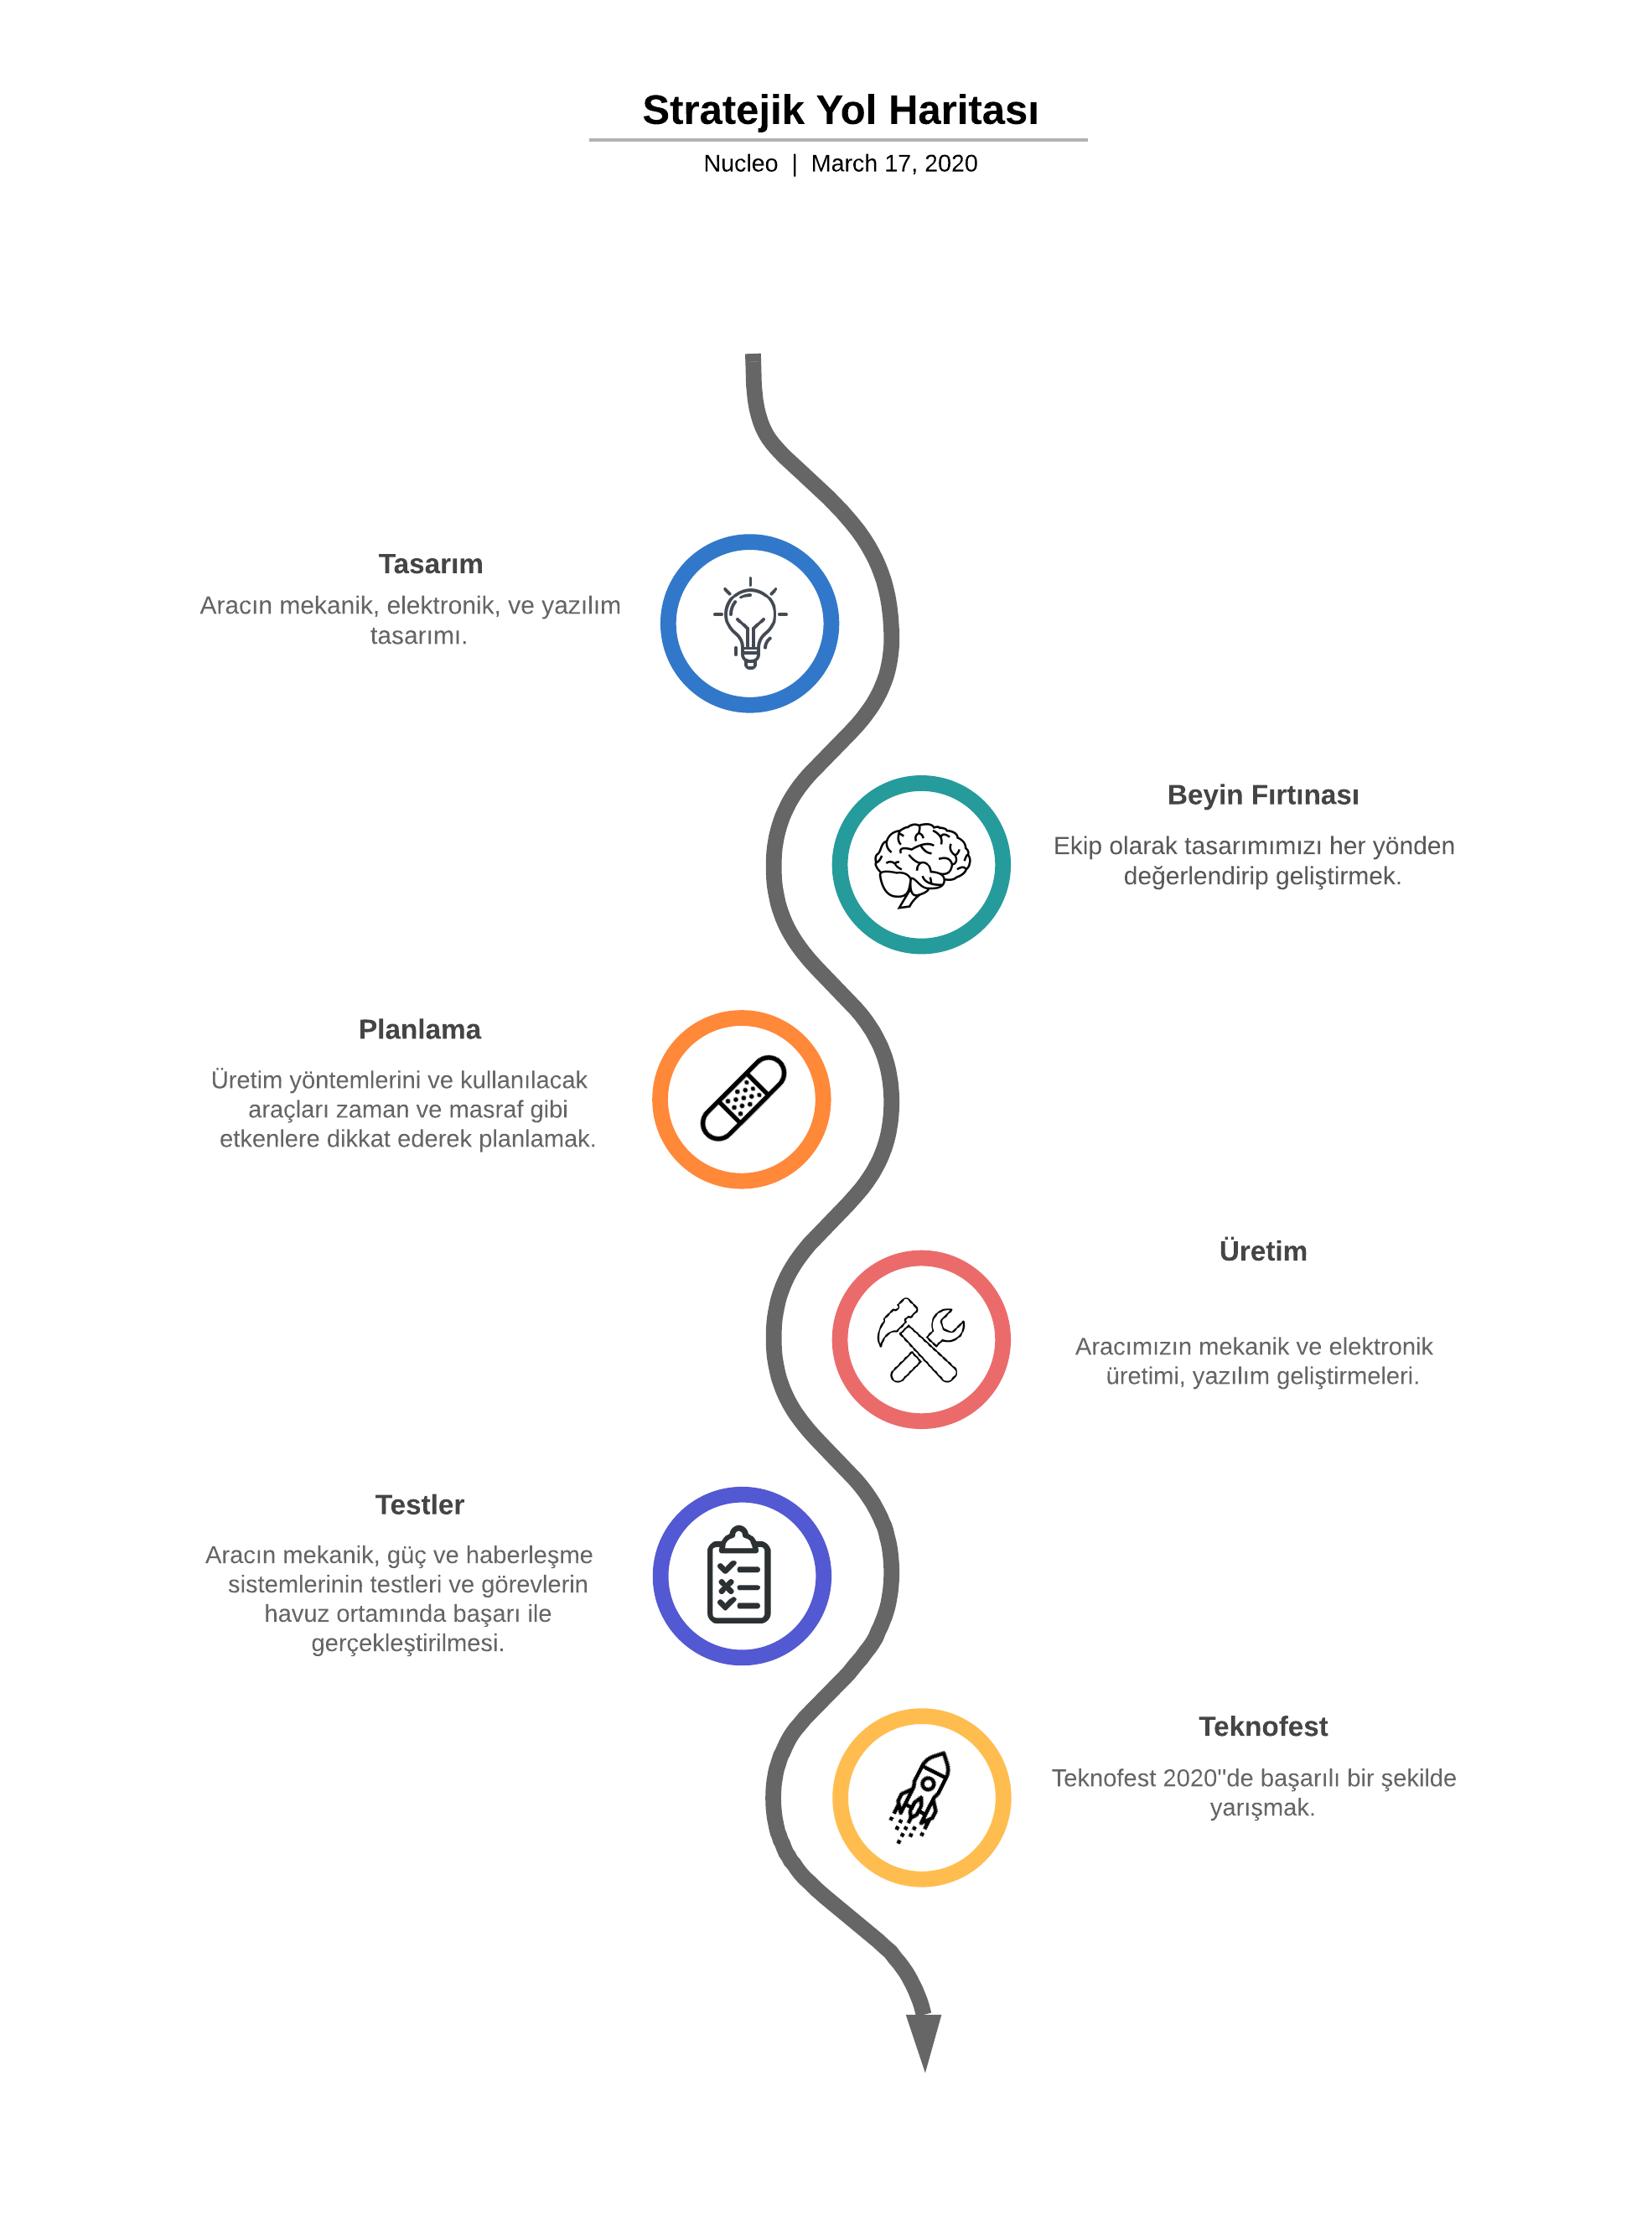
\includegraphics[width=1\textwidth]{images/timeline.png}
\caption{Stratejik Yol Haritası}
\label{fig:path}
\end{figure}

\newpage

\paragraph{} Takım üye sayısının az olması nedeniyle, görev dağılımı yapılmış olsa dahi tüm üyelerin aracın her aşamasında ortak emeği olacaktır. Her üyenin bireysel olarak sorumlu olduğu görevler bulunmaktadır.

\begin{figure}[hbt!]
\centering
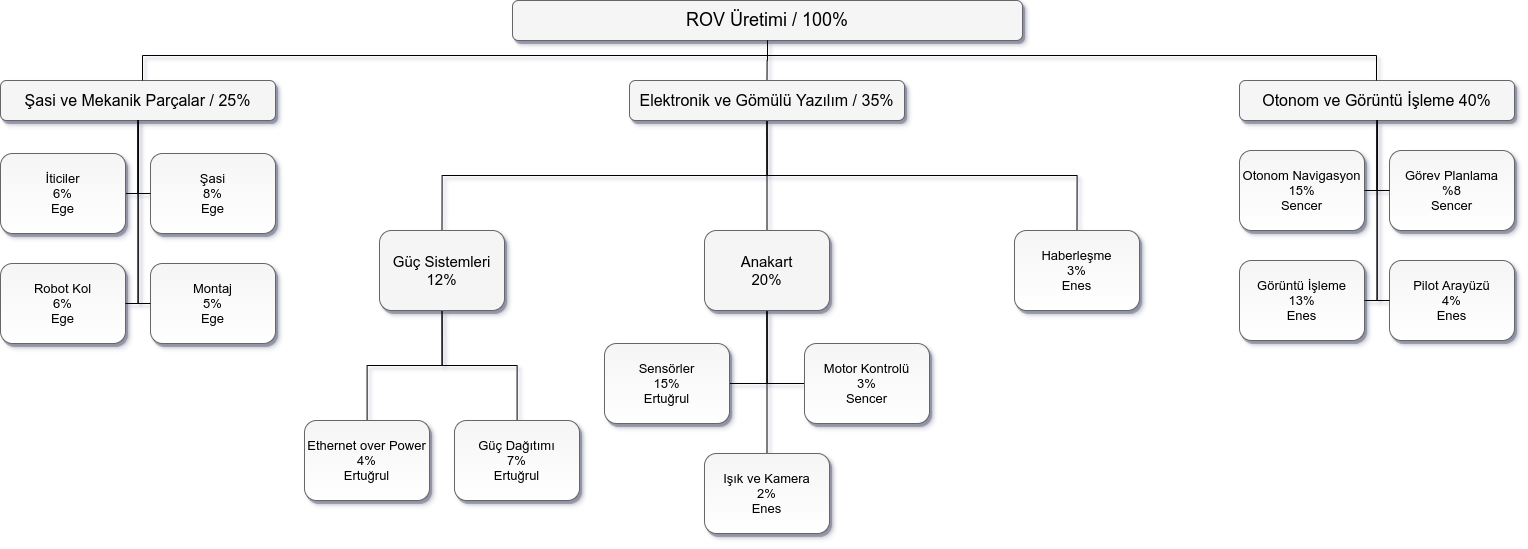
\includegraphics[width=1\textwidth]{WBS.png}
\caption{İş Dağılım Yapısı (WBS)}
\label{fig:wbs}
\end{figure}

\paragraph{} Ekip üyelerinden Enes Demirağ takımın genel organizasyonu, görüntü işleme, haberleşme sistemleri, kullanıcı arayüzü, ışık ve kamera alanlarından, Sencer Yazıcı otonom navigasyon, görev planlama ve motor kontrolör tasarımından, Ege Saygılı şasi, itici, tutucu kol tasarımı, üretimi ve montajından Sinan Ertuğrul Yıldırım sensörler, güç dağıtım sistemleri, ethernet modülü ve elektronik baskı devre tasarımından sorumludur.

\newpage

\section{Araç Ön Tasarımı}

\paragraph{} Takımımızın uzaktan kumandalı su altı araç sistemi yüzeyde bulunan bir yer istasyonu, ve aracın kendisinden oluşmaktadır. Yer istasyonunda 15.6 inç ekrana kadar dizüstü bilgisayar kullanımı desteklenmektedir. Aynı zamanda yer istasyonunda 48VDC güç kaynağı bulunmaktadır, güç kaynağı ile aracın güç beslemesi arasında 30A bir sigorta ve acil durdurma butonu bulunmaktadır. Taşınabilir yer istasyonunu prize bağlanması ve aracın da yer istasyonuna bağlanmasının ardından araç kullanıma hazır olmaktadır. Taşınabilir yüzey istayonunda aynı zamanda aracın güç ve iletişim kablosu taşınabilecektir.

\begin{figure}[hbt!]
\centering
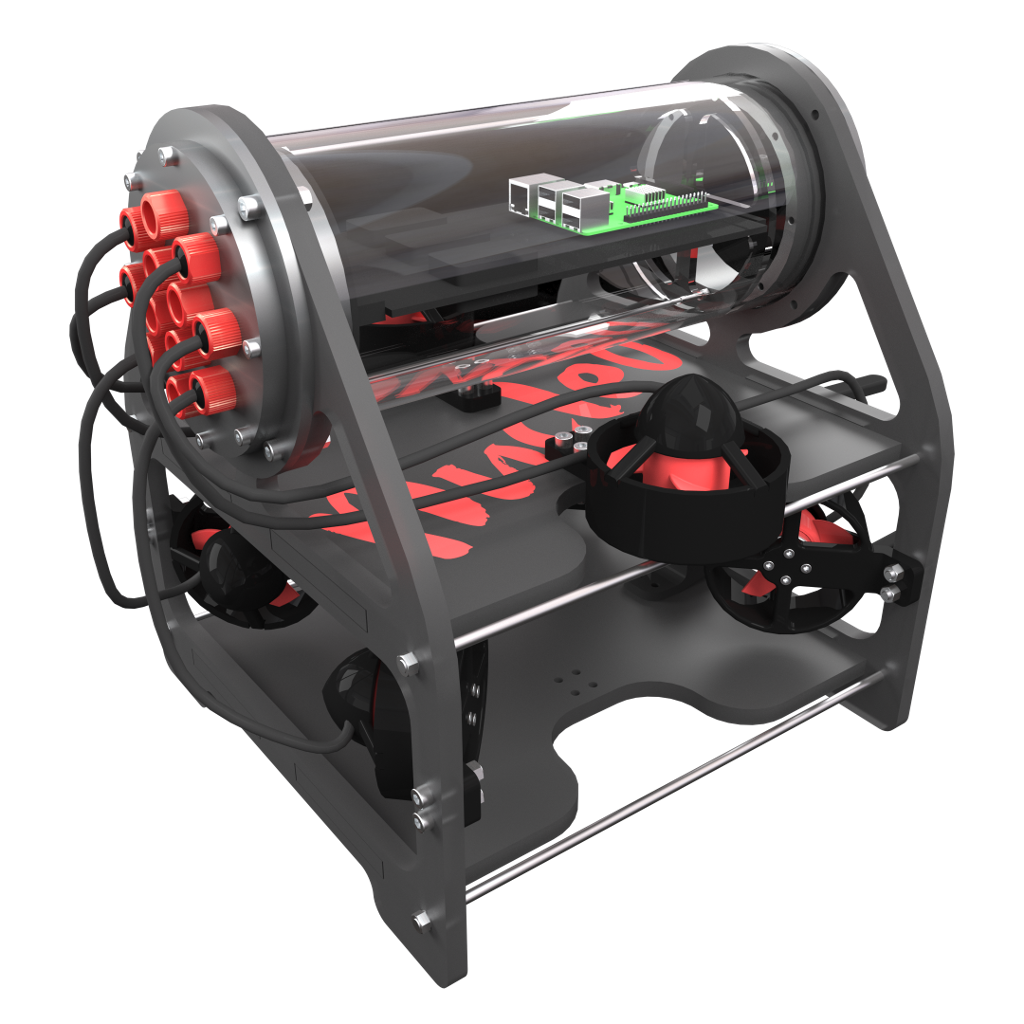
\includegraphics[width=1\textwidth]{render.png}
\caption{Aracın Render'ı}
\label{fig:render}
\end{figure}

\newpage

\paragraph{} Araç üzerinde beş eksende hareket özgürlüğü sağlaması için altı adet fırçasız motorlu itici bulunmaktadır (Şekil \ref{fig:itici}). İticiler takımımız tarafından tasarlanmıştır. Aracın elektronikleri su geçirmez akrilik bir kap içerisinde bulunmaktadır. Su geçirmez kaba kablo girişleri/çıkışları, kapak sistemleri vs. tüm su girişi olabilecek açıklıklarda o-ring conta sistemi kullanılmıştır.\cite{BOOK:o-ring} Aracın şasesi akrilik plastik (PMMA) malzemeden modüler bir yapıda tasarlanmıştır. Bu modülerlik sayesinde araç üzeri yapılması istenecek herhangi bir modifikasyon kolaylaştırılmıştır.

\begin{figure}[hbt!]
\centering
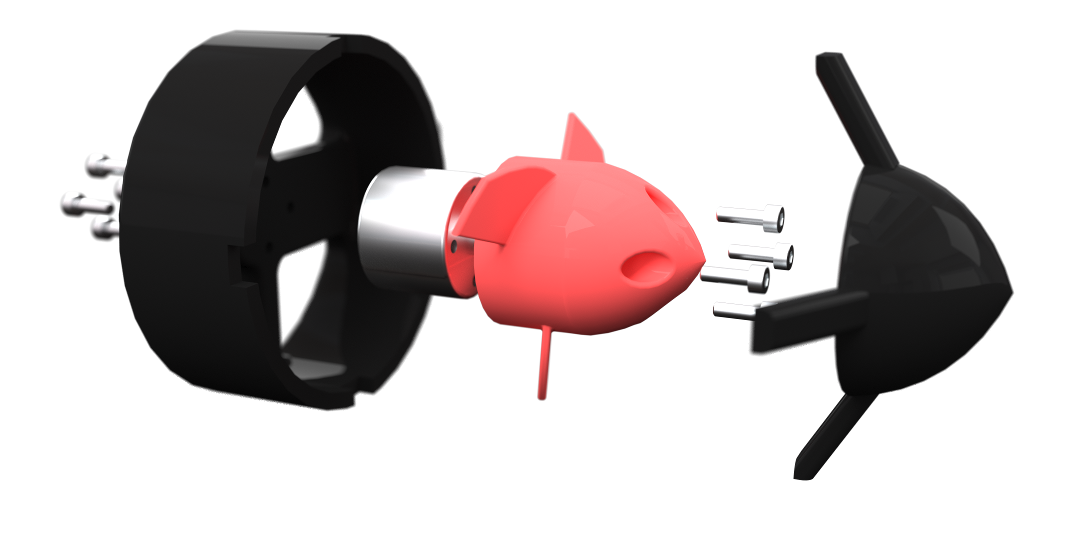
\includegraphics[width=1\textwidth]{itici.png}
\caption{Su Altı İticisi}
\label{fig:itici}
\end{figure}


\subsection{Sistem Ön Tasarımı}
\paragraph{} Sistem entegrasyon diyagramında da (Şekil \ref{fig:SID}) görüldüğü üzere, yüzey kısmında bir adet kontrol merkezi bulunmaktadır, bu taşınabilir kutu; araç kontrol bilgisayarı, araç güç kaynağı, güç kaynağı ile bağlantılı koruma (sigorta ve acil durum güç kesme butonu) vb. elemanları içerisinde barındırmaktadır. 

\paragraph{} Aracın kendisi ise, navigasyon bilgisayarı, mikroişlemci, motor sürücüler, kamera vb. elektronik elemanları içeren bir su geçirmez hazne ve suyla temas eden altı adet itici ve görev spesifik eyleyicileri içermektedir (örn. tutucu kol) (Şekil \ref{fig:gripper}).

\newpage

\begin{figure}[hbt!]
\centering
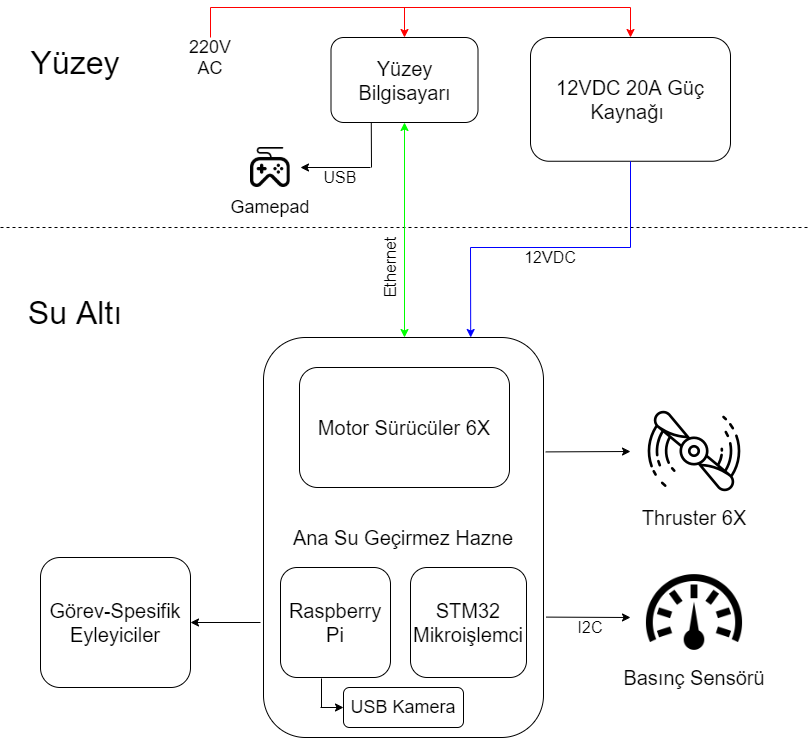
\includegraphics[width=1\textwidth]{SID.png}
\caption{Sistem Entegrasyon Diyagramı}
\label{fig:SID}
\end{figure}

\subsection{Aracın Mekanik Tasarımı}
\paragraph{} Araç, elektronik elemanları içeren ana su geçirmez hazne, şase, itici motorlar ve görev odaklı manipülatörlerden oluşmaktadır. Su geçirmez hazne silindirik yapıdadır ve arka kapağında kablo giriş/çıkışları, ön kapağında ise saydam bir kapak bulunmaktadır ve bu kapak kamera için görüş sağlamaktadır. Kapakların tüp ile arasındaki sızdırmazlığı için o-ring conta yatakları içeren iki adet flanş bulunmaktadır (Şekil \ref{fig:oring}). 

\begin{figure}[hbt!]
\centering
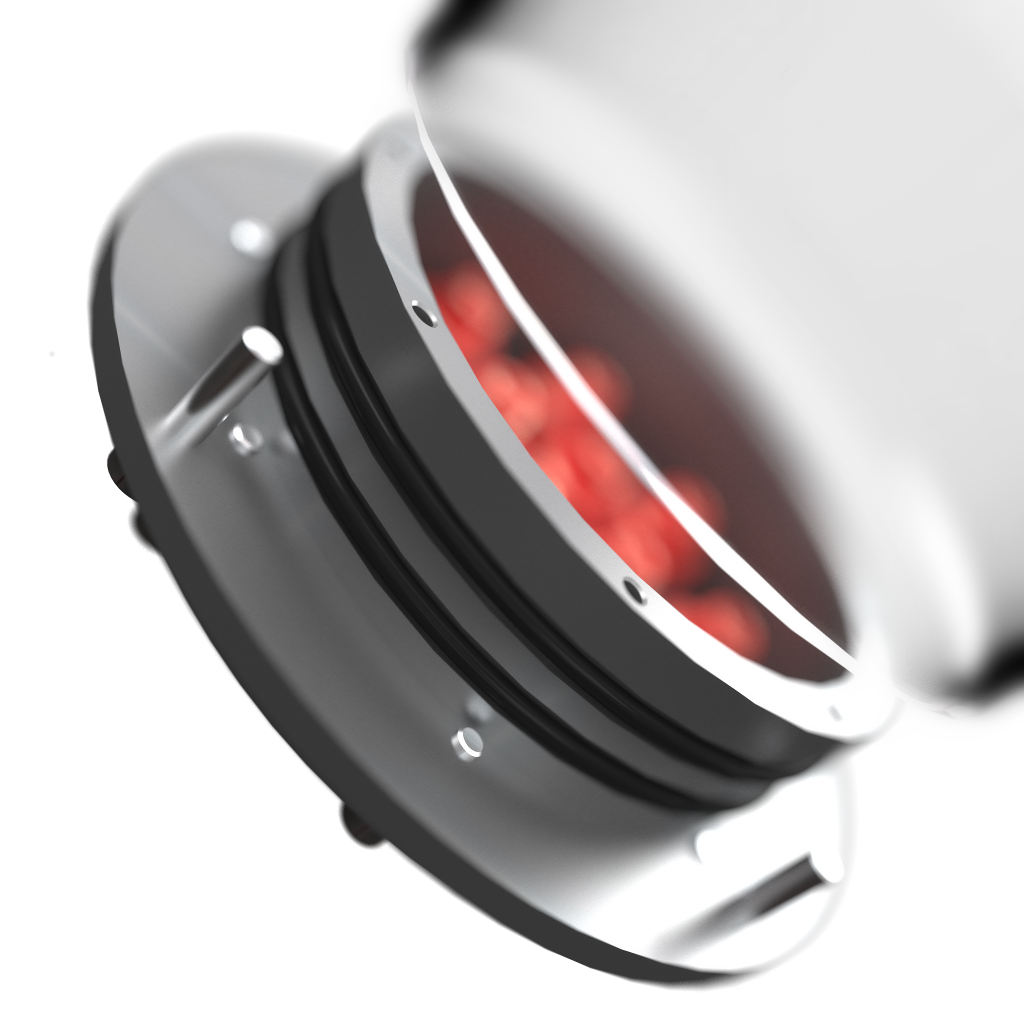
\includegraphics[width=0.4\textwidth]{oring.png}
\caption{O-Ring Conta Sızdırmazlık Sistemi}
\label{fig:oring}
\end{figure}

\newpage

\paragraph{} Aracın bütün parçalarının bağlandığı yapı olan şase ise birbine geçmeli şekilde tasarlanmış iki boyutlu akrilik plakalar şeklinde tasarlanmıştır. Bu akrilik plakaların montajı paslanmaz saplamalar ve somunlar ile yapılmıştır. Görev odaklı alet olarak yarışma görevlerinde bulunan objelerin manipülasyonu için bir adet üç parmaklı, fırçasız motor ve vidalı mil ile tahriklenen bir tutucu geliştirilmiştir. Bu tutucunun parmak sayısı ve şekli yarışma görevlerinde bulunan objelere göre değişebilecektir. 


\begin{figure}[hbt!]
\centering
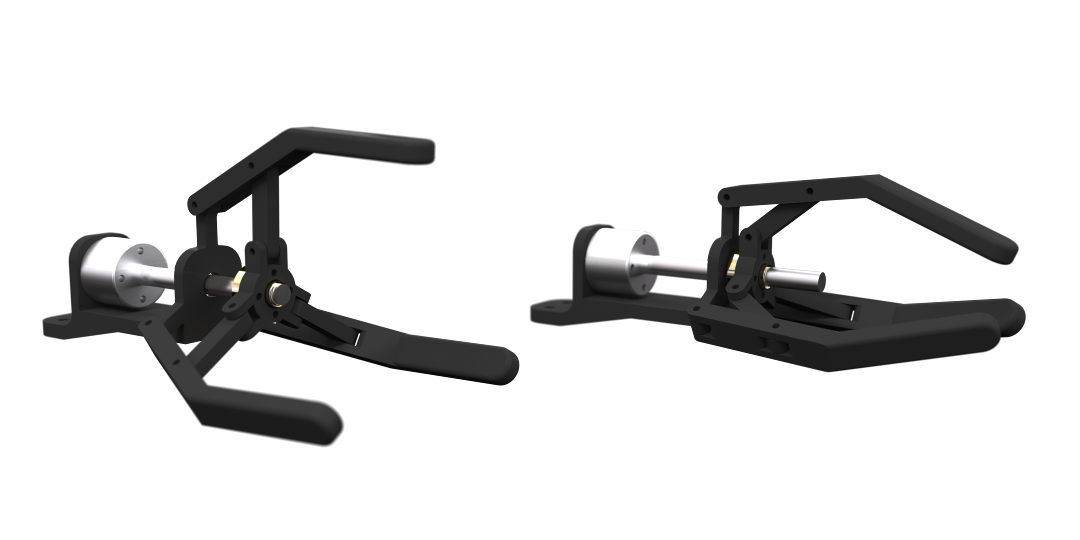
\includegraphics[width=1\textwidth]{images/gripper_render.png}
\caption{Tutucu Kol Renderı}
\label{fig:gripper}
\end{figure}

\subsubsection{Mekanik Tasarım Süreci}

\paragraph{} Aracın mekanik tasarımına, bütçe, malzeme erişim  ve işleme imkanları, yerli malzeme kullanımı, yarışma boy ve ağırlık sınırlamaları ve kullanılacak elektronik elemanların boyutlarından yola çıkılarak başlanmıştır. Kullanılması elzem olan elektronik komponentlerin ve o komponentlerin boyutlarının saptanmasının ardından aracın geri kalan ölçülerini belirleyecek olan ana su geçirmez haznenin boyutları belirlenmiştir. Su geçirmez hazne saydam olması, yarışma derinliği için yeterince dayanıklı olması, ucuz ve kolayca bulunabiliyor olmasından ötürü saydam akrilik tüp seçilmiştir.

\paragraph{} Ana haznenin belirlenmesinin ardından şase tasarımına geçilmiş ve haznenin şasede üst konumda bulunması amaçlanmıştır. Hazne, hacminden ötürü aracın yüzerliğinin büyük kısmını oluşturmaktadır, aracın yüzerlik merkezi ağırlık merkezine göre yukarıda ayarlanmaya çalışıl-mıştır (Şekil \ref{fig:moment}), bu fark sayesinde bir düzeltme momenti oluşacak ve araç serbest halde yere parelel duracaktır, ve stabilitesi artacaktır.\cite{BOOK:rovmanual} Yüzerlik merkezi ve ağırlık merkezi arasındaki farkı daha da açmak ve ağırlık merkezini iticileri hizasına getirmek için araç su geçirmez haznesi dışında diğer tüm elemanlarını alt kısımda bulunduracak şekilde tasarlanmıştır.

\newpage

\paragraph{} Şase ve su geçirmez kabın kapakları gibi aracın yüzey alanının büyük kısmını oluşturan parçalar olabildiğince düşük hidrodinamik direnç oluşturacak şekilde tasarlanmıştır. Hesaplamalı akışkanlar dinamiği gibi yöntemlerle en uygun ve düşük sürüklenme katsayısına göre tasarlamaya gerek duyulmamıştır, çünkü yüzeyden enerjisini alan uzaktan kumandalı su altı araçlarında özellikle düşük hızlarda (1 - 1.5 $m/s$) araca etki eden hidrodinamik sürüklenme kuvveti, aracın güç ve haberleşme kablosu (tether) tarafından uygulanan kuvvete göre çok düşük kalmaktadır.\cite{BOOK:rovmanual} Bu sebeple sürüklenme kuvveti konusunda aracın tasarımında optimizasyona gerek duyulmamıştır.

\begin{figure}[hbt!]
\centering
 \begin{adjustbox}{width=10cm}
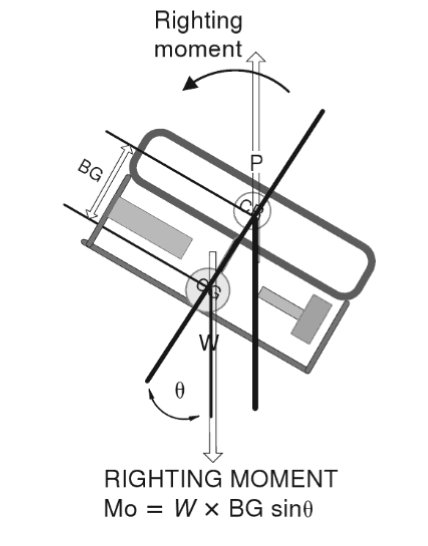
\includegraphics[width=1\textwidth]{moment.png}
 \end{adjustbox}
%  \vspace{-1cm}
\caption{Düzeltme Momenti}
\label{fig:moment}
\end{figure}


\subsubsection{Malzemeler}

\paragraph{} Aracın iskeletini (şasi) oluşturan parçalar ve su geçirmez haznenin tüpü gibi parçalar akrilik (PMMA) malzemeden seçilmiştir. Akrilik; hazır tüp bulunmasının kolaylığı, plaka halinde bulunmasının kolaylığı, lazer kesiminin çok kolay bulunuyor olması, ekonomik olması ve görsel özellikleri gibi sebeplerden ötürü seçilmiştir. İtici motorların koruyucu kısımları, pervaneler ve tutucu manipülatör gibi parçalar 3B plastik basım yöntemiyle üretilecektir. Su geçirmez haznenin o-ring conta bulunduran flanş parçaları alüminyumdan seçilmiştir. Araçta sabitleme elemanı olarak paslanmaz alyan başlı civatalar, paslanmaz somun ve gijonlar kullanılacaktır. Suda bulunması gereken kablo birleşim yerleri kablo gömme reçinesi ile gömülecek ve kablo üzerinde  sızdırmazlık sağlanacaktır (Şekil \ref{fig:inlinesplice}).

\newpage

\begin{figure}[hbt!]
\centering
 \begin{adjustbox}{width=10cm}
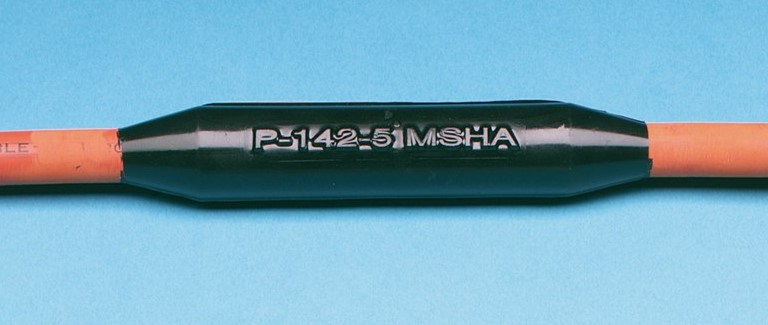
\includegraphics[width=1\textwidth]{inlinesplice.jpg}
 \end{adjustbox}
\caption{Reçine İle Korunmuş Bir Kablo Eki}
\label{fig:inlinesplice}
\end{figure}

\subsubsection{Üretim Yöntemleri}

\paragraph{} Aracın şasesini oluşturan akrilik parçalar lazer kesim yöntemi ile işlenecektir. Bu yöntem ve akrilik malzeme seçimi üretim kolaylığı ve ekonomik oluşundan dolayı tercih edilmiştir. Su geçirmez kabın conta yataklı flanşı aluminyumdan manuel torna da talaşlı imalat yöntemiyle işlenecektir. 3B plastik parçalar 3B yazıcılar yardımıyla basılacaktır.

\paragraph{} İticilerde kullanılan fırçasız motorlar tuzlu ve tatlı suda çalışabilmektedir. Ancak bu motorlarda kullanılan malzemelerin bazıları (aluminyum motor şasesi) suda uzun süre korozyona uğramadan çalışabilmesine rağmen bazı malzemeler (bakır bobinlerin sarıldığı demir çekirdek, çelik rulman, neodymium mıknatıslar vb.) ise zaman içerisinde korozyona uğramakta ve motorun bozulmasına sebep olmaktadır (Şekil \ref{fig:korozyon}.a). Bu sebeple motorların rulmanlarının pirinç burç ya da seramik/plastik rulmanlarla değiştirilmesi ve bobinlerin sarıldığı demir çekirdeğin tamamının epoksi gibi koruyucu plastiklerle kaplaması planlanmaktadır. (Şekil \ref{fig:korozyon}.b). 

\begin{figure}[hbt!]%
% \vspace{-3cm}
    \centering
    \subfloat[Korozyona Uğramış Motor Örneği]{{\includegraphics[width=7cm]{korozyon.png} }}%
    \qquad
    \subfloat[Korozyona Karşı Korunma Önlemleri Alınmış Motor Çekirdeği]{{\includegraphics[width=6cm]{potted.png} }}%
    \caption{Fırçasız Motorlarda Korozyon}%
    \label{fig:korozyon}%
\end{figure}

% \begin{figure}[hbt!]
% \centering
%  \begin{adjustbox}{width=7cm}
% \includegraphics[width=1\textwidth]{images/korozyon.png}
%  \end{adjustbox}
% \caption{Fırçasız Bir Motorda Korozyon Örneği}
% \label{fig:korozyon}
% \end{figure}

% \begin{figure}[hbt!]
% \centering
%  \begin{adjustbox}{width=7cm}
% \includegraphics[width=1\textwidth]{images/potted.png}
%  \end{adjustbox}
% \caption{Korozyona Karşı Korunma Önlemleri Alınmış Bir Motor Çekirdeği}
% \label{fig:potted}
% \end{figure}

\newpage
\subsubsection{Fiziksel Özellikler}

\begin{figure}[hbt!]
\centering
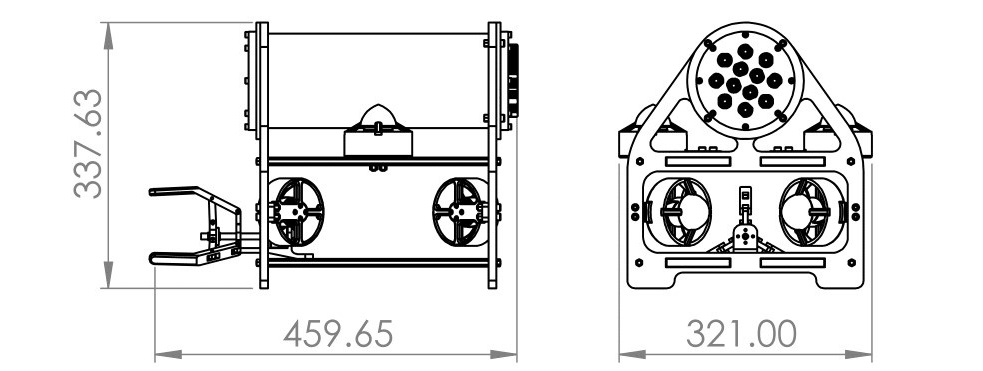
\includegraphics[width=1\linewidth]{images/specs.jpg}
\caption{Su Altı Aracının Ölçüleri}
\label{fig:technicaldrawing}
\end{figure}


\paragraph{} Aracın ölçüleri 32cm genişlik, 34cm yükseklik ve 46cm uzunluk şeklindedir. Aracın ağırlığı ve yüzerliği 6.8kg dır, bu sayede araç hafifçe pozitif bir yüzerliğe sahiptir, herhangi bir kontrol kaybında araç hafif yüzerliği sayesinde yüzeye çıkacak ve sudan geri alınabilecektir. 


\subsection{Elektronik, Algoritma ve Yazılım Tasarımı}

\subsubsection{Elektronik Ön Tasarım Süreci}

\paragraph{} Aracın testlerine erken başlayabilmek adına elektronik tasarımda ilk olarak temel bileşenleri barındıran ve esneklik sağlayabilecek baskı deve tasarlanmaya başlanacaktır. Anakartta önceden düşünülmüş ve kullanılacak olan güç dağıtımı, haberleşme ve sensör pinlerinin dışında yedek planlara hızlı geçiş için fazladan giriş ve çıkışlar bulundurulacaktır. İlk testlerin ardından eksik ve hatalı noktalar giderilerek devremiz güncellenecek ve bu süreç istenilen görevleri başarıyla gerçekleştirene kadar devam edecektir. 

\subsubsubsection{Enerji İletimi ve Dağıtımı}

\paragraph{} Araç, gücünü şebekeden gelen 220VAC gerilimi 48VDC'ye dönüştüren bir güç kaynağından alacaktır. Araca ulaşan güç, regülatör yardımıyla 12V'a dönüştürülecektir. Enerji iletimi sırasında direkt 12V yerine 48V kullanılmasının sebebi iletimdeki akımı ve geirlim düşümünü azaltmaktır. Aracın altı motoru ve diğer elektronik devrelerinin güç gereksinimi göz önüne alındığında yaklaşık 350 Watt gücü 48V'ta taşıyabilmek için 14AWG kablo yeterli olacaktır. 14AWG, bakır, 30m kabloda 10A'da yaklaşık 5V gerilim düşümü olacaktır. 
\newpage
\paragraph{}Yüzey bilgisayarı ile aracın haberleşmesi güç kabloları üzerinden sağlanacak ve bu sayede haberleşme için ekstra kablo ihtiyacına gerek duyulmayaaktır. Araca aktarıp 12V'a düşürülen gücün bir kısmı doğrudan motor sürücüler ve motorlara iletilirken, bir kısmı regülatörler tarafından istenilen gerilimlere ayarlanıp ilgili bileşenlere dağıtılacaktır. Güç dağıtımı, hazırlanan güç dağıtım kartı üzerinden gerçekleştirilecektir.

\subsubsubsection{Temel Bileşenler}

\paragraph{} Aracın elektronik devreleri bir anakart ve tüp içerisindeki alanı verimli kullanabilmek adına anakart üzerine takılı yardımcı kartlardan oluşacaktır. Su altında çalışma performansı kanıtlanmış olan altı adet fırçasız doğru akım motoru, yine altı adet ESC ile sürülecektir. ESC'ler vasıtasıyla motorları kontrol edecek, görev eyleyici elemanları kontrol edecek ve gerekli sensörlerden veri alıp mikroişlemciyle haberleşerek aracın kontrolünü sağlayacak bir \href{https://www.st.com/en/microcontrollers-microprocessors/stm32f429zi.html}{STM32F429ZI} mikrodenetleyicisi kullanılacaktır. STM32 mikrodenetleyicileri yüksek performanslı, takım üyeleri tarafından sıkça kullanılan mikrodenetleyiciler olup, araç için uygun görülmüştür. 

\paragraph{} Aracın üst seviye yazılım görevlerini gerçekleştirilebilmesi adına, yeterli performansı ile \href{https://www.raspberrypi.org/products/raspberry-pi-3-model-b}{Raspberry Pi} kullanılacaktır. Yer istasyonu ile Raspberry Pi, ethernet üzerinden haberleşecektir. Pilotun istediği hareketlerin motorlar tarafından gerçekleştirilmesi ise Raspberry Pi'ın, mikrodenetleyici ile UART üzerinden haberleşmesiyle sağlanacaktır.


\subsubsubsection{Yardımcı Bileşenler}

\paragraph{} Raspberry Pi tarafından işlenecek görüntü, bir USB kamera vasıtasıyla alınacaktır. Aracın suyun ne kadar altında durduğunu anlaması adına bir basınç sensörü, istenilen görevleri gerçekleştirebilmesi adına bir tutucu kol bulunacaktır. Tutucu kol yine STM32 tarafından bir motor sürücü vasıtasıyla kontrol edilecektir.

\subsubsection{Algoritma Ön Tasarım Süreci}


\paragraph{} Araç uzaktan kontrol ve otonom olmak üzere iki farklı modda çalışabilecektir. Su Altı Temizlik ve Su Altı Montaj görevlerinde araç tamamen pilot kontrolünde olduğu süre boyunca kamera görüntüleri ve sensör verilerini yüzey kontrol sistemi arayüzünde görüntülerken, pilot joystick yardımıyla aracın navigasyonunu sağlayacaktır. Bunun dışında takım tarafından geliştirilen PID kontrolör sayesinde araç, pilot müdahale etmediği sürecek bulunduğu son derinliği koruyacaktır.

\paragraph{} Engel Geçiş ve Denizaltı Tespit görevleri pilot müdahalesi olmadan tamamen otonom olarak hareket edecektir. Görüntü işleme algoritması ile göreve yönelik hedefler tespit edilecek ve güdüm kontrolü ile su altı navigasyon sağlanacatır. Bu süre içerisinde yer istasyonu ile olan uzaktan kontrol sistemi pasif duruma geçecek ve gözlem amaçlı olarak tek yönlü bir şekilde kamera görüntüleri ve sensör verileri yüzeye aktarılacaktır.
\newpage

\begin{figure}[hbt!]
\centering
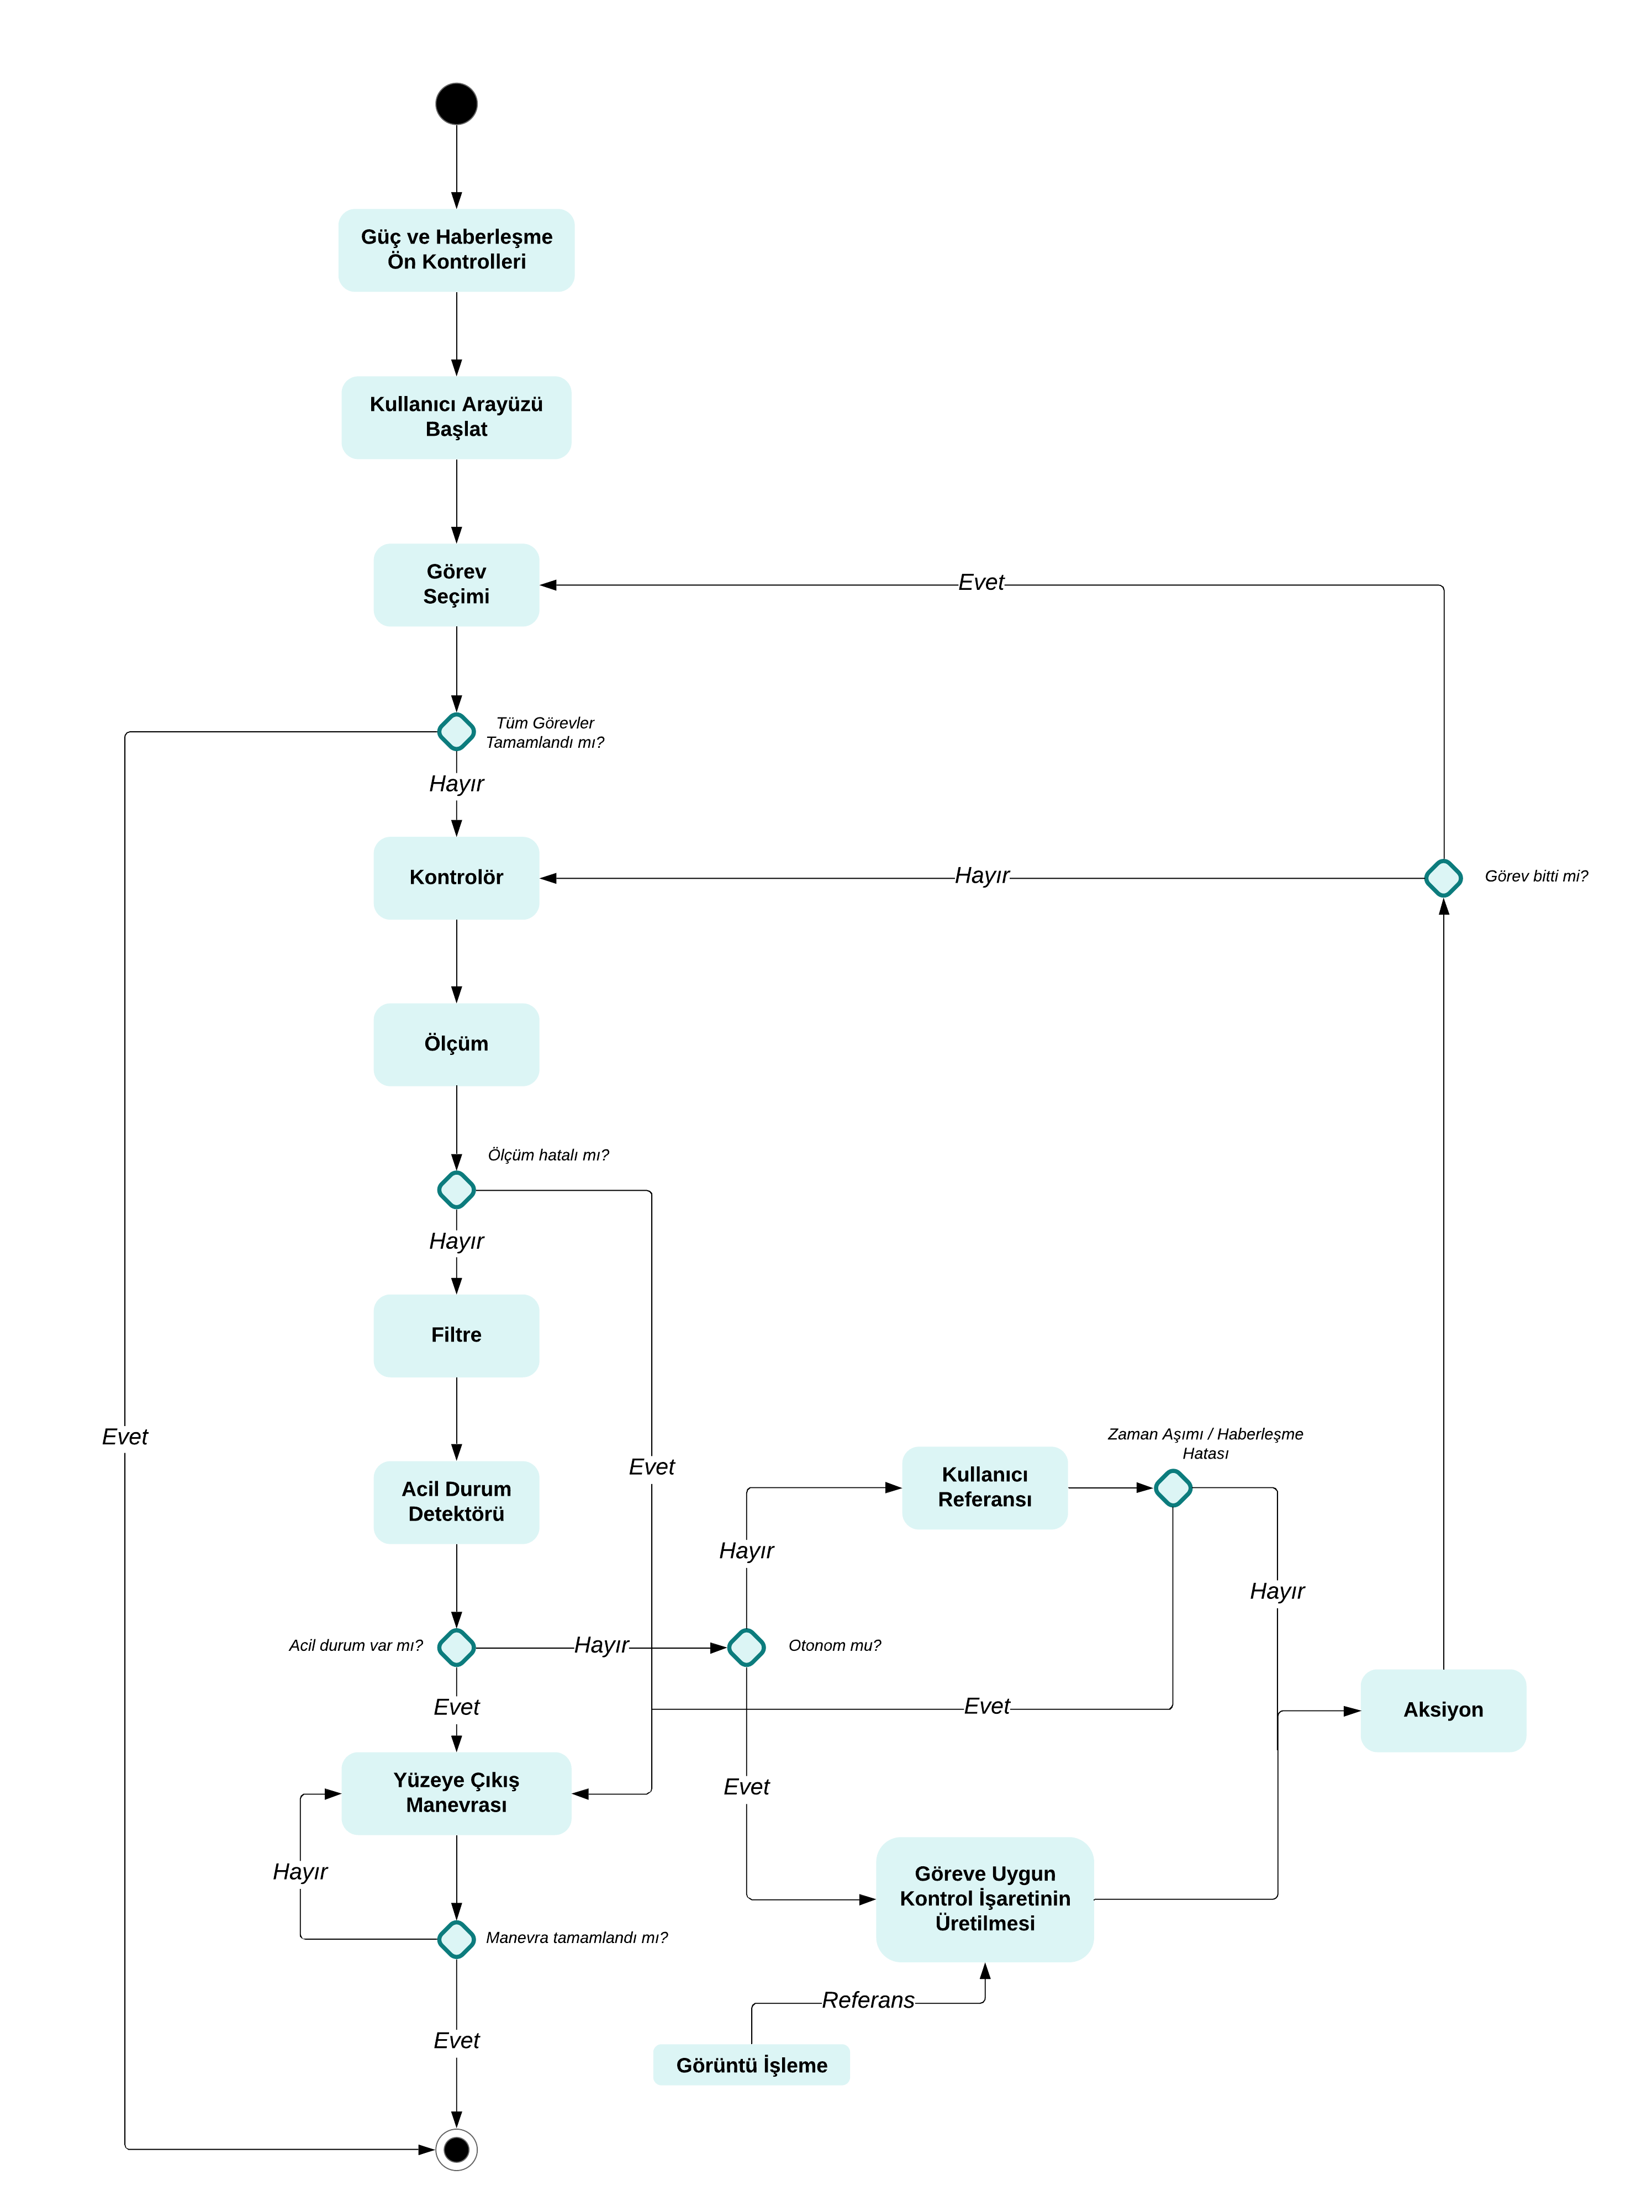
\includegraphics[width=0.95\textwidth]{flowchart-v2.png}
\caption{Akış Diyagramı}
\label{fig:flow-chart}
\end{figure}

\paragraph{} Araç üzerindeki tüm kontrol, görüntü işleme ve karar verme algoritmaları ROS üzerinde Durum Makinesi (State Machine) methodu ile gerçeklenmektedir. ROS hakkında detaylı bilgi 3.3.3.2'de verilmiştir.

\newpage
\subsubsection{Yazılım Ön Tasarım Süreci}


\paragraph{} Yazılım ekibi üyesi Sencer Yazıcı aynı zamanda İTÜ AUV Takımı yazılım ekip liderliğini üstlendiğinden, İTÜ AUV Takımı bünyesinde geliştirilen yazılımın kullanılması hedeflenmektedir. Takımda geliştirilen yazılım, modüler bir altyapı içerdiğinden, kolayca entegre edilebilecektir.

\paragraph{} Başlıca sistemin genel parçalara ayrılması gerekirse;
\begin{itemize}
    \item STM32 mikrodenetleyici üzerinde çalışacak olan gömülü sistem, alt seviye yazılım.
    \item Raspberry Pi Üzerinde çalışacak olan, karar verme mekanizmasına ve haberleşme sistemlerine sahip sistem, üst seviye yazılım.
    \item Yer istasyonunda çalışacak olan, operatör komutlarının aracın komuta sistemine aktarılmasını sağlayan haberleşme çift yönlü telemetri (veri aktarımı).
\end{itemize}

\subsubsubsection{Gömülü Sistem \& Mikrodenetleyici}

 \paragraph{}  Anakart üzerine takılı STM32 mikrodenetleyicinin temel görevi alt seviye elektronik işlemleri ve aracın temel fonksiyonlarını kontrol etmektir. Geliştirilen gömülü yazılım, güç hattının gerilimini hassas bir şekilde ölçerek motorları istenilen kuvveti üretecek şekilde bir PWM sinyali üretir. Burada, ekibimiz tarafından motorun su altında yapılan testleriyle elde edilen PWM - Kuvvet karakteristiği kullanılır. bu sayede test edilen gerilim aralığında herhangi bir gerilimde, mikrodenetleyici istenilen kuvveti üretecek PWM sinyaini hesaplayabilir, ve böylece 5-Eksen PID kontrolör ile kontrol sistemi çalıştırılır. Burada SimScape üzerinde yapılan CFD testleri ile de, drag (direnç) ve damping (sönüm) katsayıları hesaplanır. Bu hesaplar sonucu elde edilen matematik modele göre bir PID kontrolör tasarlanır, ve su altında gerçek sistem üzerinde yapılan testler sonucu ince ayar (Fine Tuning) yapılarak nihai parametrelere ulaşılır. 

\paragraph{} Ayrıca gömülü sistem, basınç sensöründen elde ettiği veriyi, Kalman Filtresi ile filtreleyerek 5 eksen kontrol sisteminde kullanılacak olan derinlik geribeslemesini hesaplar. Bunun yanı sıra, yine temel fonksiyonlar kategorisine giren, eyleyicilerin (manipülatörlerin) kontrolünü de, gömülü yazılım yürütür.

\paragraph{} Son olaraksa, tüm bu verilerin ve kontrol sistemlerinin, temel karar verme mekanizmasının bulunduğu ana bilgisayara iletilmesi içinse, istenirse Ethernet, isternirse UART kullanılabilir. Gömülü sistem bu iletişim yöntemlerinin hangisinin aktif olduğunu belirleyerek birinden ötekine dinamik olarak geçebilmektedir. Gömülü yazılım tüm bunları, \href{https://www.ros.org}{ROS} topic ağı üzerinde gerçekleştirmekte olup, herhangi bir topic'i dinleyebilir, herhangi bir topic'e veri aktarımı yapabilmektedir. 

\newpage

\paragraph{} Bu gömülü sistem, yazılım ekibi üyemiz tarafından İTÜ AUV Takımı bünyesinde geliştirilmiştir ve tamamen özgündür. Bu yazılım İTÜ AUV Takımında da aktif olarak kullanılmaktadır ve modüler yapısı sayesinde teknofest yarışması için de kolayca entegre edilebilecektir.


\subsubsubsection{Merkezi Bilgisayar ve Karar Mekanizması Sistemi}

\paragraph{} Aracın temel fonksiyonları gömülü yazılım tarafından STM32 üzerinde gerçekleştirilirken, görev akışını ve üst seviye hesaplamaları gerçekleştirecek olan bilgisayar, Raspberry Pi 2, Ethernet ve ya UART üzerinden STM32 ile haberleşerek temel fonksiyonların üst seviye yazılımlar ile iletişimini sağlar. Üst seviye yazılımlarda, ROS ağı üzerinde çalışacak olan yazılımlar, görüntü işleme ve HD USB Kamera görüntüsünün yüzeye aktarılması bulunur.

\paragraph{} ROS ağı üzerinde bulunan Node'lar, temel olarak veri iletişimi, acil durum kontrolü, görüntü işleme sonucu elde edilen verileri işleme ve gerekli durumlarda tespit edilen objelerin pozisyon ve oryantasyon tespiti (tahmini) ve bu pozisyon(lar)ın filtrelenmesi gibi konuları gerçekleştirir.

\subsubsubsection{Görüntü İşleme}
\paragraph{} Araç üzerindeki kameralardan alınan görüntü Raspberry Pi üzerinde çalışan bir Python programı ile işlenip analiz edilerek, araca otonom olarak görev odaklı kontrol işareti üretilecek ve üretilen bu çıktı referans olarak mikrodenetleyiciye iletilecektir. Görüntü işleme sisteminde openCV kütüphanesi kullanılacaktır. Elde edilen kamera görüntüsü su altında optimize edilecek görüntü işleme filtrelerinden\cite{ARTICLE:image_proc} geçirilecek ve geliştirdiğimiz görev karar algoritması sonucu yer istasyonundan tamamen bağımsız olarak, otonom bir şekilde görevleri gerçekleştirecektir.


\subsubsection{Dış Arayüzler}
\paragraph{} ROS ağının TCP/IP üzerinden çalışıyor olmasının avantajlarından faydalanarak, Rqt tabanlı bir kullanıcı arayüzü (GUI) geliştirmeyi düşünmekteyiz. Bu sayede yüzeydeki bilgisayar, Raspberry Pi'ın IP adresi ile, $11311$ numaralı porttan ROS ağına bağlanabilecek ve ROS ağı üzerindeki tüm topic'leri dinleyebilecek ve ya bu topic'lere veri aktarabilecektir. İTÜ AUV Takımı için oluşturmuş olduğumuz örnek bir kullanıcı arayüzü Şekil \ref{fig:gui}'de verilmiştir.
\newpage
\begin{figure}
\centering
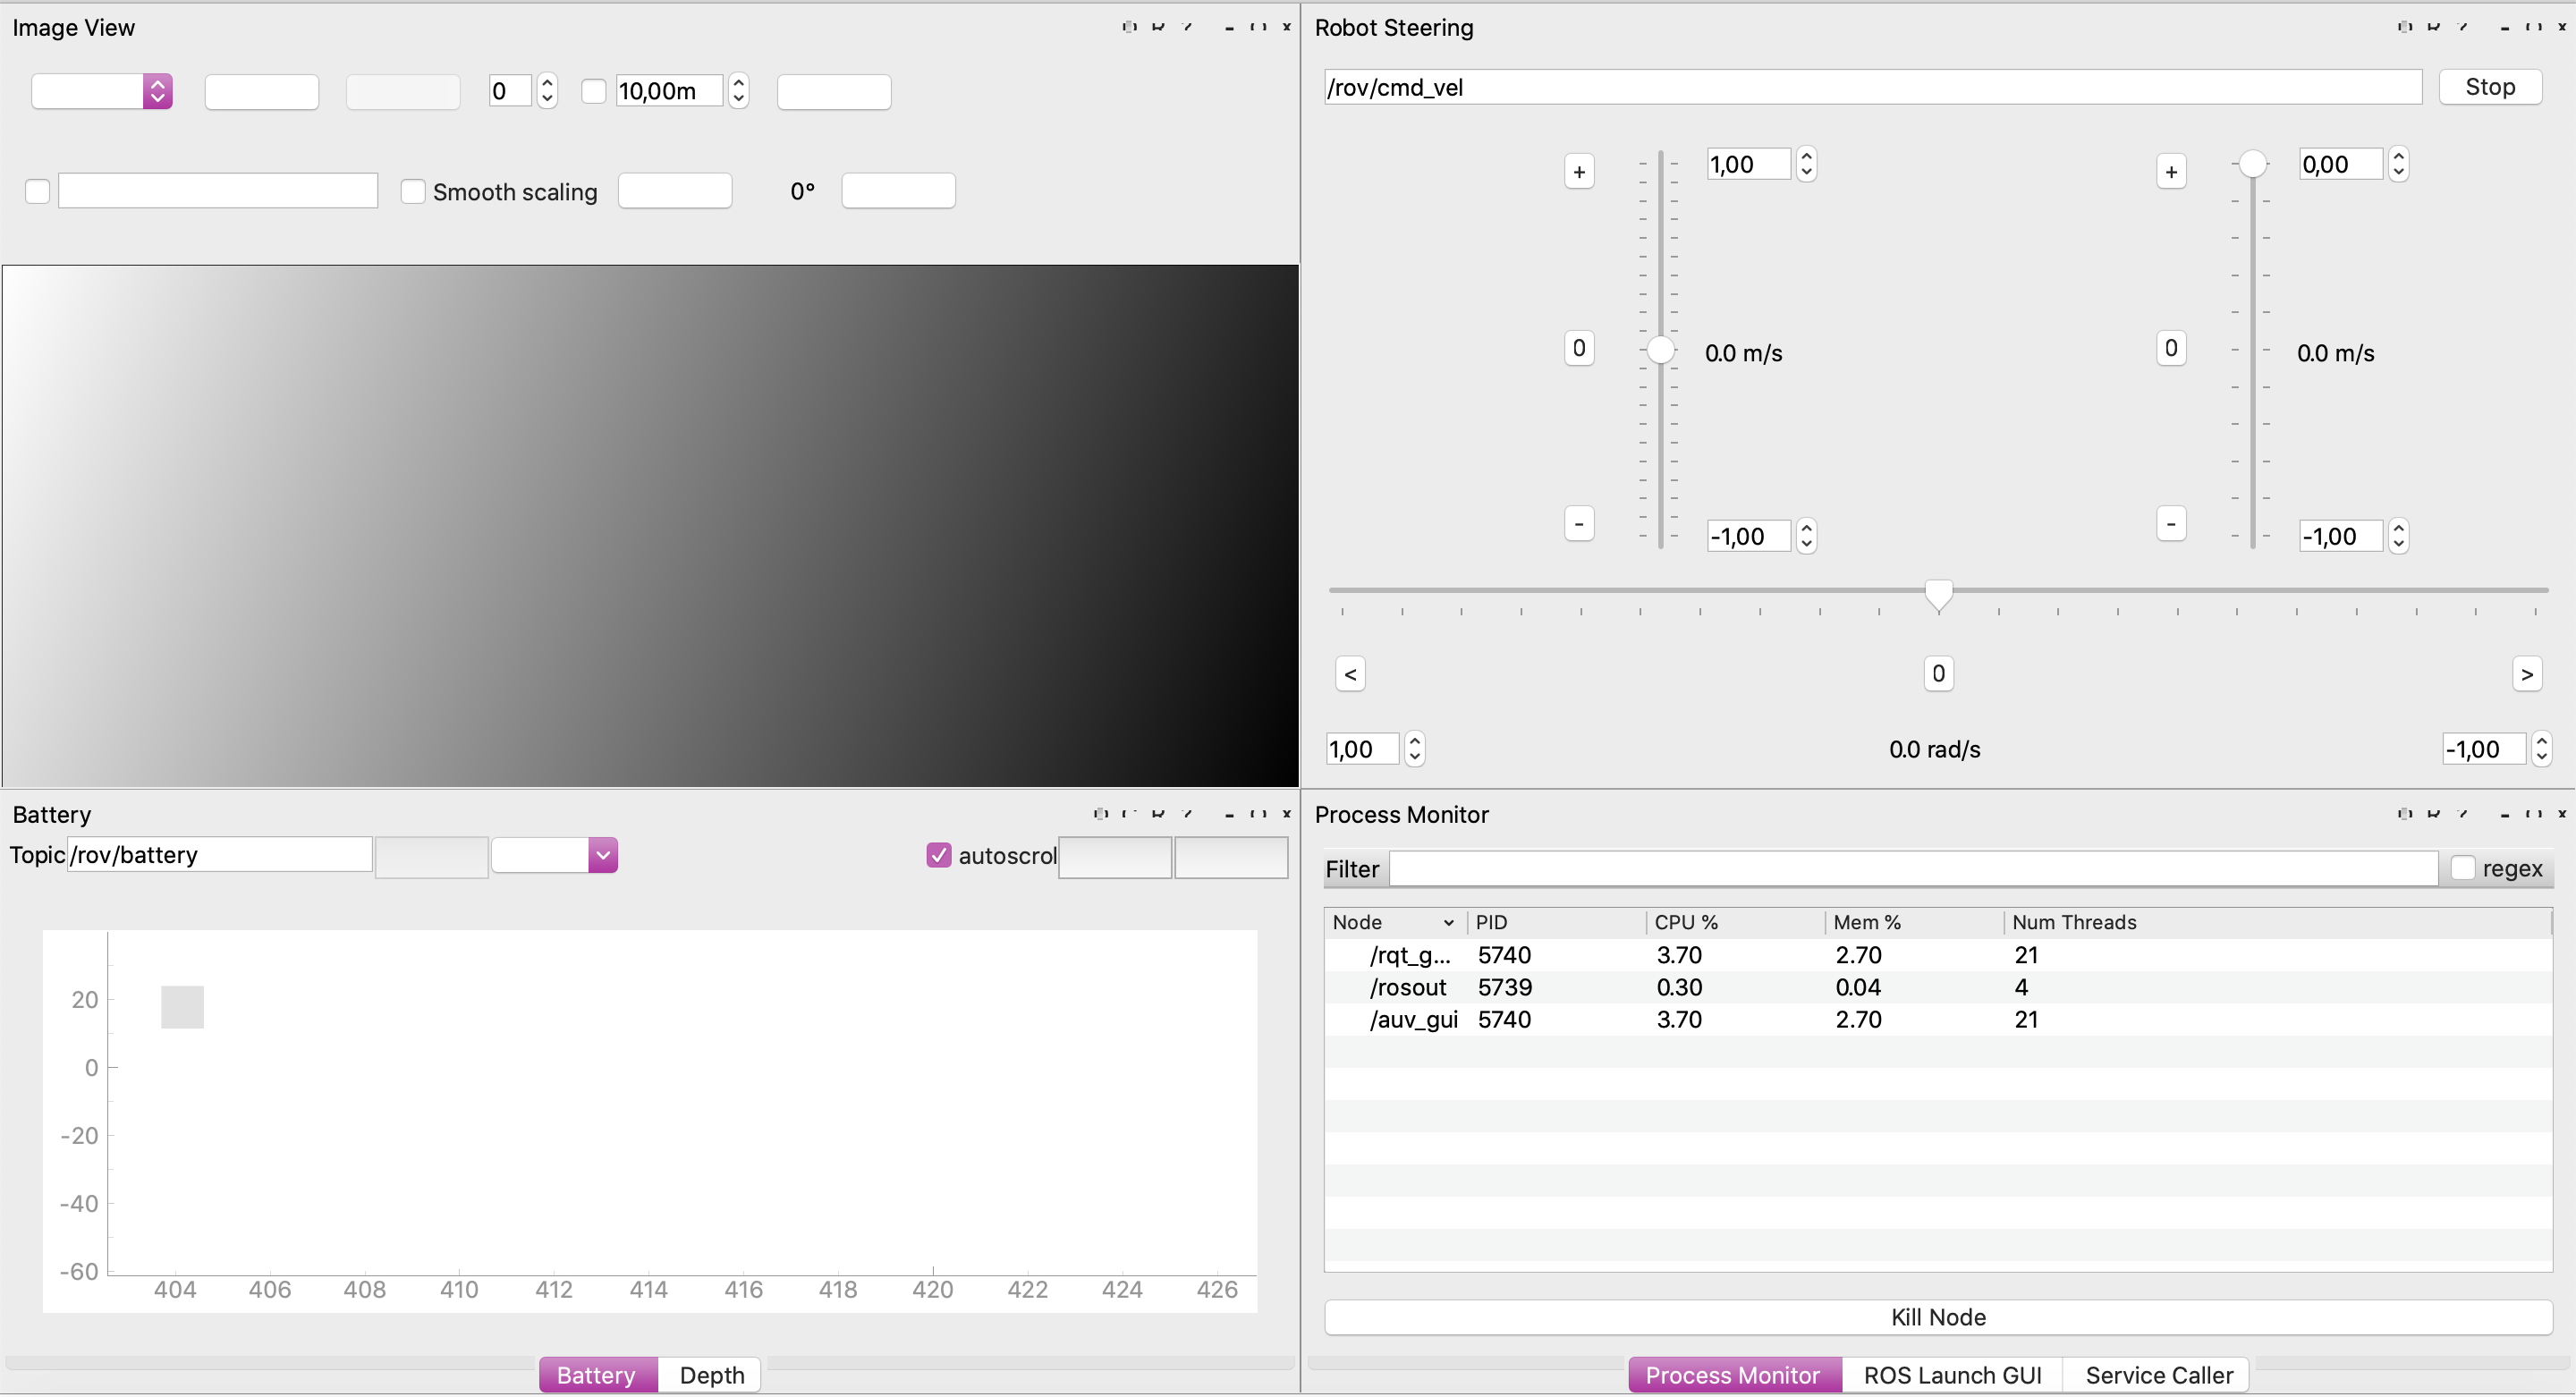
\includegraphics[width=1\textwidth]{images/gui.png}
\caption{Örnek Kullanıcı Arayüzü (GUI)}
\label{fig:gui}
\end{figure}


\section{Güvenlik}

\paragraph{}Aracın tasarımı gibi teknik, üretim ve montaj gibi pratik işlerin yanı sıra verilen en büyük öncelik iş güvenliği ve emniyetdir. Testlerde ve atölye çalışmalarında öncelik, çalışmak için güvenli ve konforlu alanı oluşturmak olacaktır. Atölye çalışmalarında kişisel koruyucu ekipmanlar olan gözlük, eldiven vb. ekipmanların kullanılmasının yanı sıra ilk yardım kiti bulundurulması da ihmal edilmeyecektir.

\paragraph{}Aracın üzerindeki motorlar, dışarıdan zarar görmeyecek ve dışarıya zarar vermeyecek şekilde konumlandırılmıştır. Bunların yanı sıra, aracın üzerinde kullanılacak tüm plastik kelepçeler kullanıcılara zarar veremeyecek şekilde tıraşlanacak ve aracın üzerinde herhangi bir sivri uç bırakılmayacaktır. Aracın su altında herhangi bir sorunda karşılaşılması durumunda yer istasyonunda bulunan acil durdurma butonu sayesinde aracın hızlı bir şekilde durdurulma imkanı bulunmaktadır. Dağıtım hatlarında uygun sigortalar ve koruma devreleri de kullanılacaktır. İnsan sağlığına zarar verecek yüksek gerilimlere çıkılmayacaktır.

\newpage

\section{Zaman, Bütçe ve Risk Planlaması}
\subsection{Zaman Planlaması}
\paragraph{} Proje zaman planlaması aşamasında ekip üyelerinin müsaitlik durumları, üniversite sınavları, yarışma son teslim tarihleri, ulusal ve uluslararası ekonomik ve sağlık koşulları göz önüne alınmıştır. 

\begin{figure}[hbt!]
\centering
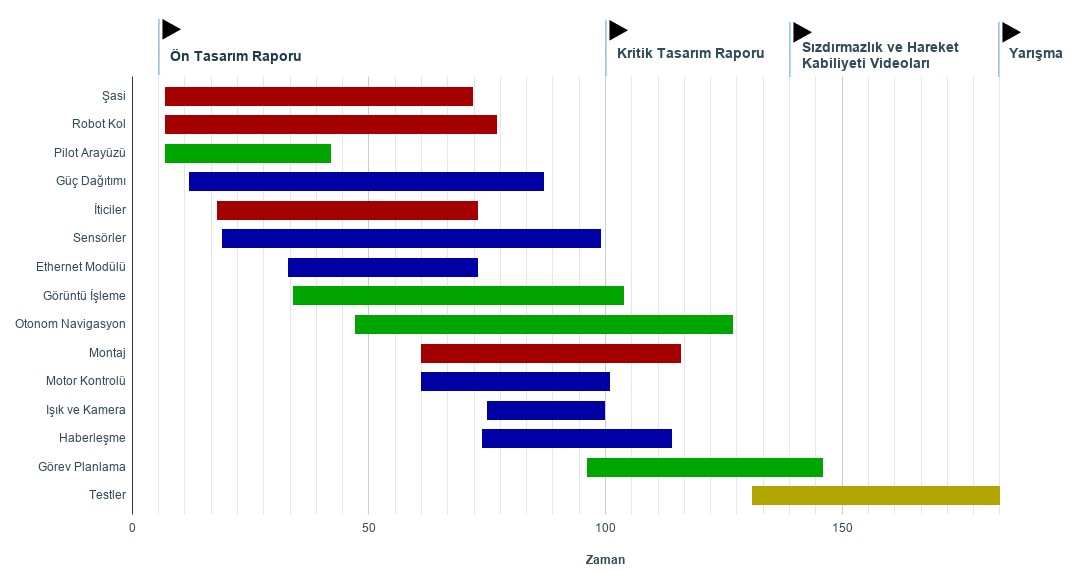
\includegraphics[width=1\textwidth]{chart-final.png}
\caption{Zaman Çizelgesi}
\label{fig:gantt-chart}
\end{figure}

\begin{table}[hbt!]
\centering
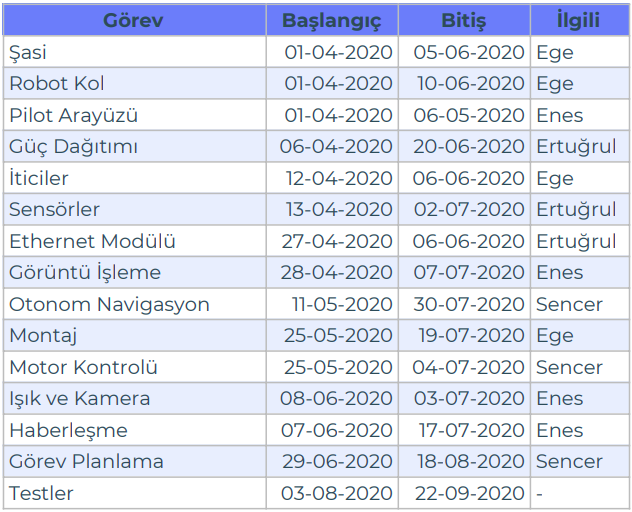
\includegraphics[width=0.6\textwidth]{data.png}
\caption{Tahmini İş-Zaman Planı}
\label{fig:data}
\end{table}

\newpage
\subsection{Bütçe Planlaması}

\paragraph{} Bütçe planlaması aşamasında araç üzerindeki malzemelerde mümkün oldukça yüksek kalite ve düşük maliyet hedeflemekteyiz.

\begin{table}[hbt!]
\centering
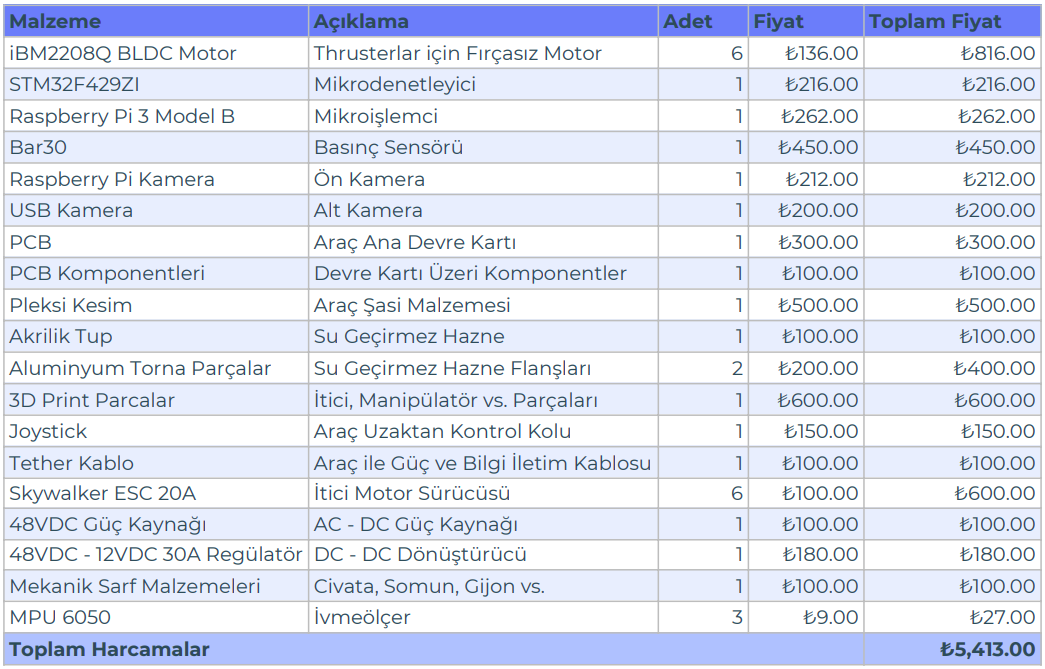
\includegraphics[width=1\textwidth]{budget.png}
\caption{Bütçe}
\label{fig:butce}
\end{table}

\subsection{Risk Planlaması}

\paragraph{} Proje geliştirme aşamalarında yaşanabilecek riskler aşağıda belirtilmiştir, ancak takımın bu robotik ve özellikle su altı araçları alanlarındaki tecrübeleri ile proje zamanında başarıyla tamamlanacaktır.

\begin{itemize}
    \item Coronavirus nedeniyle proje planlanandan daha uzun sürebilir.
    \item Yurt dışı malzeme temininde yaşanacak sıkıntılara alternatif çözüm aramak gerekebilir.
    \item Projenin beklenenden daha maliyetli olması ekonomik sorunlara neden olabilir.
\end{itemize}
\newpage
\section{Özgünlük}

%% Buraları unutmamak için öylesine yazdım. düzelticem.
\paragraph{} Geliştirdiğimiz özgün çalışmalardan birkaçı aşağıdadır.
% @enes
\begin{itemize}
    % QGroundcontrol link ve ya referans.
    \item Bir çok takımın aksine QGroundControl Programı yerine ROS ile uyumlu esnek bir kullanıcı arayüzü kullanılacaktır.
    
    \item Popüler kullanıma sahip olan PixHawk Kontrolörü yerine, ARM tabanlı bir STM32 mikrodenetleyici üzerinde tamamen kendi tasarımımız olan bir gömülü yazılım kullanılacaktır.
    %Ertuğrul: ben yazdım bunu belki silebilirsiniz.
    \item Aracın, yer istasyonu ile haberleşmesini sağlayacak ethernet kablosu, güç kablosu ile birleştirilerek tek hat üzerinden gerçekleştirilecek ve böylece kablo sayısı azalacaktır.
    
    % @ege
    \item Kendi iticilerimizi geliştirmekteyiz, iticilerimizde suda oluşabilecek korozyon etkilerine karşı gerekli koruma önlemleri alınacaktır. Bu sayede iticilerimiz proje için ekonomik olmakla birlikte uzun ömürlü ve güvenilir olacaktır. 
\end{itemize}

% REFERANS YAPILABILECEKSEK YAPALIM
\newpage
\section{Referanslar}
\vspace{-1cm}
\printbibliography[title={\textbf{ }}]


\end{document}
